% Generated by thesis/ch7/exp2/networks.py -- do not edit by hand.
\begin{sidewaysfigure}
  \centering
  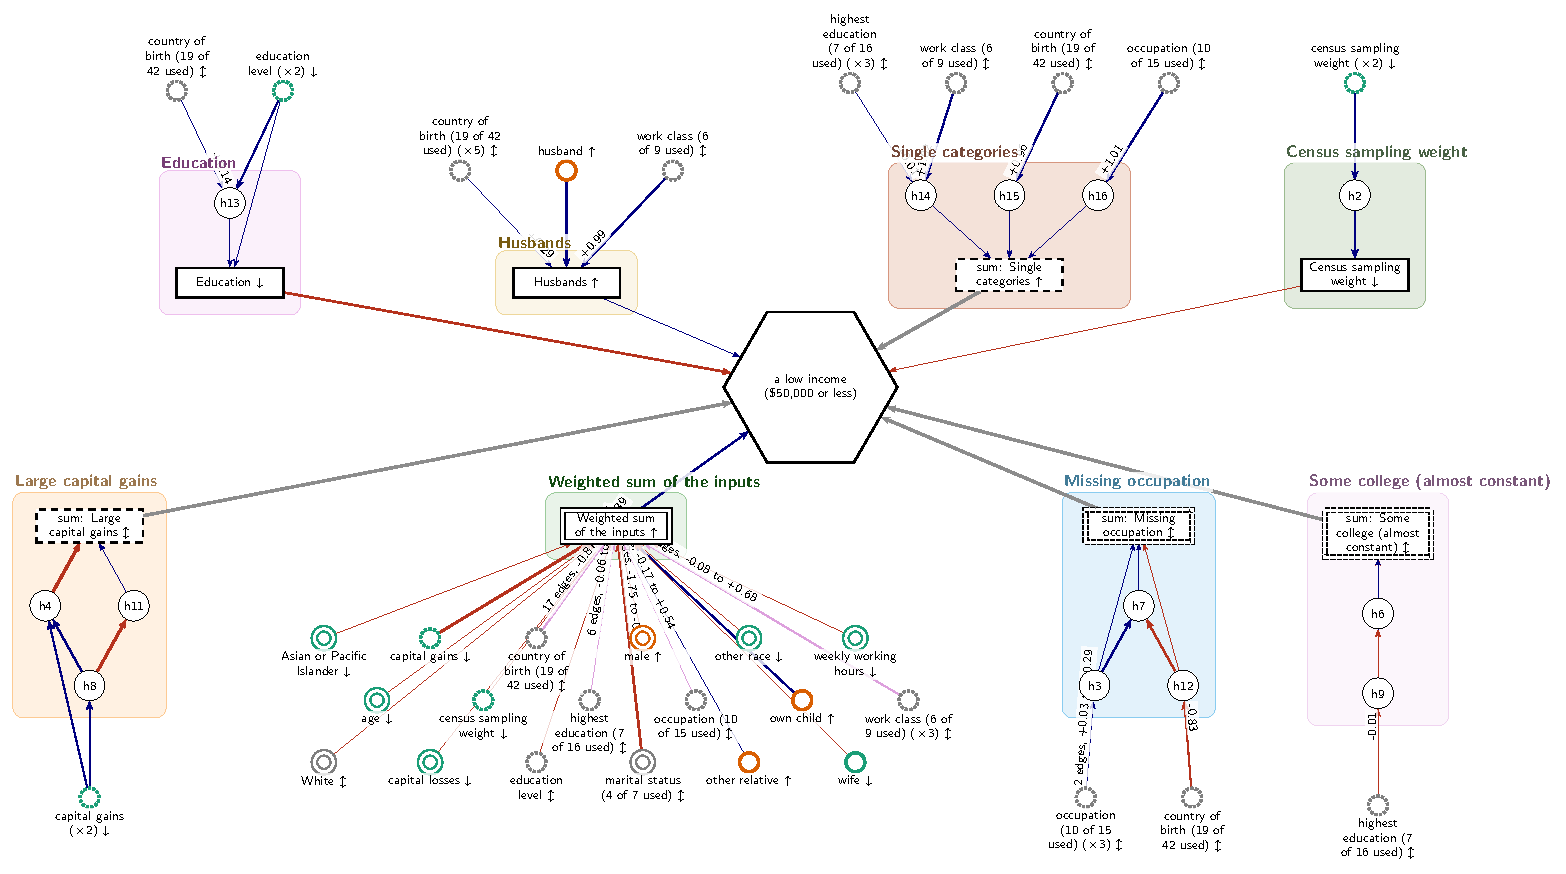
\includegraphics[width=\textheight,height=0.78\textwidth,keepaspectratio]{figures/exp2/networks/adult-s2-explained}
  \caption{Adult, seed 2 (adult-s2): every unit and connection of the explained model, nested by part. Shaded clusters are the 9 parts of the agent's explanation (8 leaf and 1 composition annotations, after 9 node splits and 1 identity nodes) and darker boxes the parts inside them; circles are hidden units; each cluster's rectangle is its output, a dashed `sum' an addition the next unit does; the hexagon is the model's output. An input used by several parts is drawn under each of them (dotted outline). Blue: positive weight (raises the score); red: negative weight (lowers it); thicker: larger weight. Orange outline and up arrow: raises the final prediction; teal and down arrow: lowers it; grey and double arrow: depends.}
  \label{fig:exp2-net-adult-s2-explained}
\end{sidewaysfigure}
